\chapter{hls4ml Synthesis and Hardware Results}
\label{ch:hls4ml-results}

\section{Synthesis Goal}
\label{sec:synthesis-goal}

The CNN models from Chapter~\ref{ch:cnn-pipeline} are useful only if they can be mapped to practical FPGA hardware. The goal of this chapter is to evaluate whether the trained classifiers can become deployment-path checkers with acceptable latency and resource overhead.

We use hls4ml to convert trained CNN models into hardware designs~\cite{duarte2018fast,aarrestad2021fast}. The synthesis flow takes a trained Keras or QKeras model~\cite{coelho2020qkeras}, generates an HLS implementation, validates the generated design with C simulation, and produces latency and resource estimates after synthesis. The final W8A8 candidates are trained with QKeras quantization-aware training before hls4ml conversion, so the software model already uses the quantized weight and activation behavior evaluated by the hardware flow. The final candidates are then evaluated in terms of added latency and added FPGA resources relative to the Coyote baseline.

The main hardware metrics are LUT usage, BRAM usage, DSP usage, and added inspection latency. The main detection metrics are accuracy, F1, true positive rate, false positive rate, and ROC AUC. The final design point should balance both groups of metrics.

\section{hls4ml Flow}
\label{sec:hls4ml-flow}

The hardware flow starts from a trained CNN. The model is exported and passed to hls4ml. hls4ml generates C++ code and an HLS project. We then run C simulation to check that the generated model produces outputs consistent with the software model. After this parity check, the design is synthesized and evaluated.

The flow is:

\begin{center}
\small
\begin{tabular}{c}
\textbf{trained CNN} $\rightarrow$ \textbf{hls4ml conversion} $\rightarrow$ \textbf{C simulation} \\[3pt]
$\rightarrow$ \textbf{HLS synthesis} $\rightarrow$ \textbf{latency and resource report}
\end{tabular}
\end{center}

This flow is repeated for selected CNN candidates. We do not synthesize every software model. Larger software models can improve F1, but they can also produce hardware designs that are too slow or too resource-heavy. The synthesis stage therefore acts as a filter between high-quality software models and deployable FPGA checkers.

\section{Hardware Tuning Parameters}
\label{sec:hls4ml-knobs}

The main hls4ml tuning parameters are quantization, reuse factor, synthesis strategy, and manual per-layer configuration.

Quantization controls the precision of weights and activations. Lower precision can reduce hardware cost, but it can also reduce model quality or create numerical differences between the software model and the generated HLS model.

The reuse factor controls how much hardware is shared across operations. A low reuse factor increases parallelism and reduces latency. It also increases resource usage. A high reuse factor uses fewer resources but increases latency.

The synthesis strategy controls whether hls4ml optimizes more aggressively for latency or resource usage. We also use manual per-layer tuning because a single global setting is often too coarse. Some layers dominate latency, while others dominate BRAM or DSP usage.

Table~\ref{tab:hls4ml-knobs} summarizes the main knobs.

\begin{table}[t]
    \centering
    \caption{hls4ml tuning parameters used during synthesis.}
    \label{tab:hls4ml-knobs}
    \begin{tabular}{p{0.25\linewidth} p{0.45\linewidth} p{0.20\linewidth}}
        \toprule
        \textbf{Parameter} & \textbf{Effect} & \textbf{Main tradeoff} \\
        \midrule
        Quantization &
        Sets weight and activation precision &
        Quality vs. area \\
        \midrule
        Reuse factor &
        Controls hardware sharing across operations &
        Latency vs. area \\
        \midrule
        Strategy &
        Selects resource-oriented or latency-oriented mapping &
        Area vs. speed \\
        \midrule
        Per-layer tuning &
        Adjusts important layers individually &
        Practical fit \\
        \bottomrule
    \end{tabular}
\end{table}

\section{Latency and Resource Tradeoff}
\label{sec:hls4ml-tradeoff}

The HLS exploration shows a clear tradeoff between detection quality, latency, and resource usage. Larger input resolutions preserve more bitstream detail and improve software F1. They also increase the cost of the hardware checker. Lower reuse factors reduce latency but require more parallel hardware. Higher reuse factors reduce hardware use but increase latency.

Figure~\ref{fig:hls-tradeoff} shows the W8A8 P50 resource-strategy sweep. Circles and squares show reuse-factor sweeps for the 256$\times$7 and 512$\times$7 models. The starred points show the manually tuned v1 candidates used for deployment evaluation. These manual candidates keep the same reported F1 as the corresponding resource-strategy sweep while reducing latency and LUT utilization.

\begin{figure}[t]
    \centering
    % Source image copied from ../ml_deep_bitstream_inspection/hls4ml/results/selected_feasible_candidates_resource_strategy/plots/latency_lut_f1_tradeoff.png
    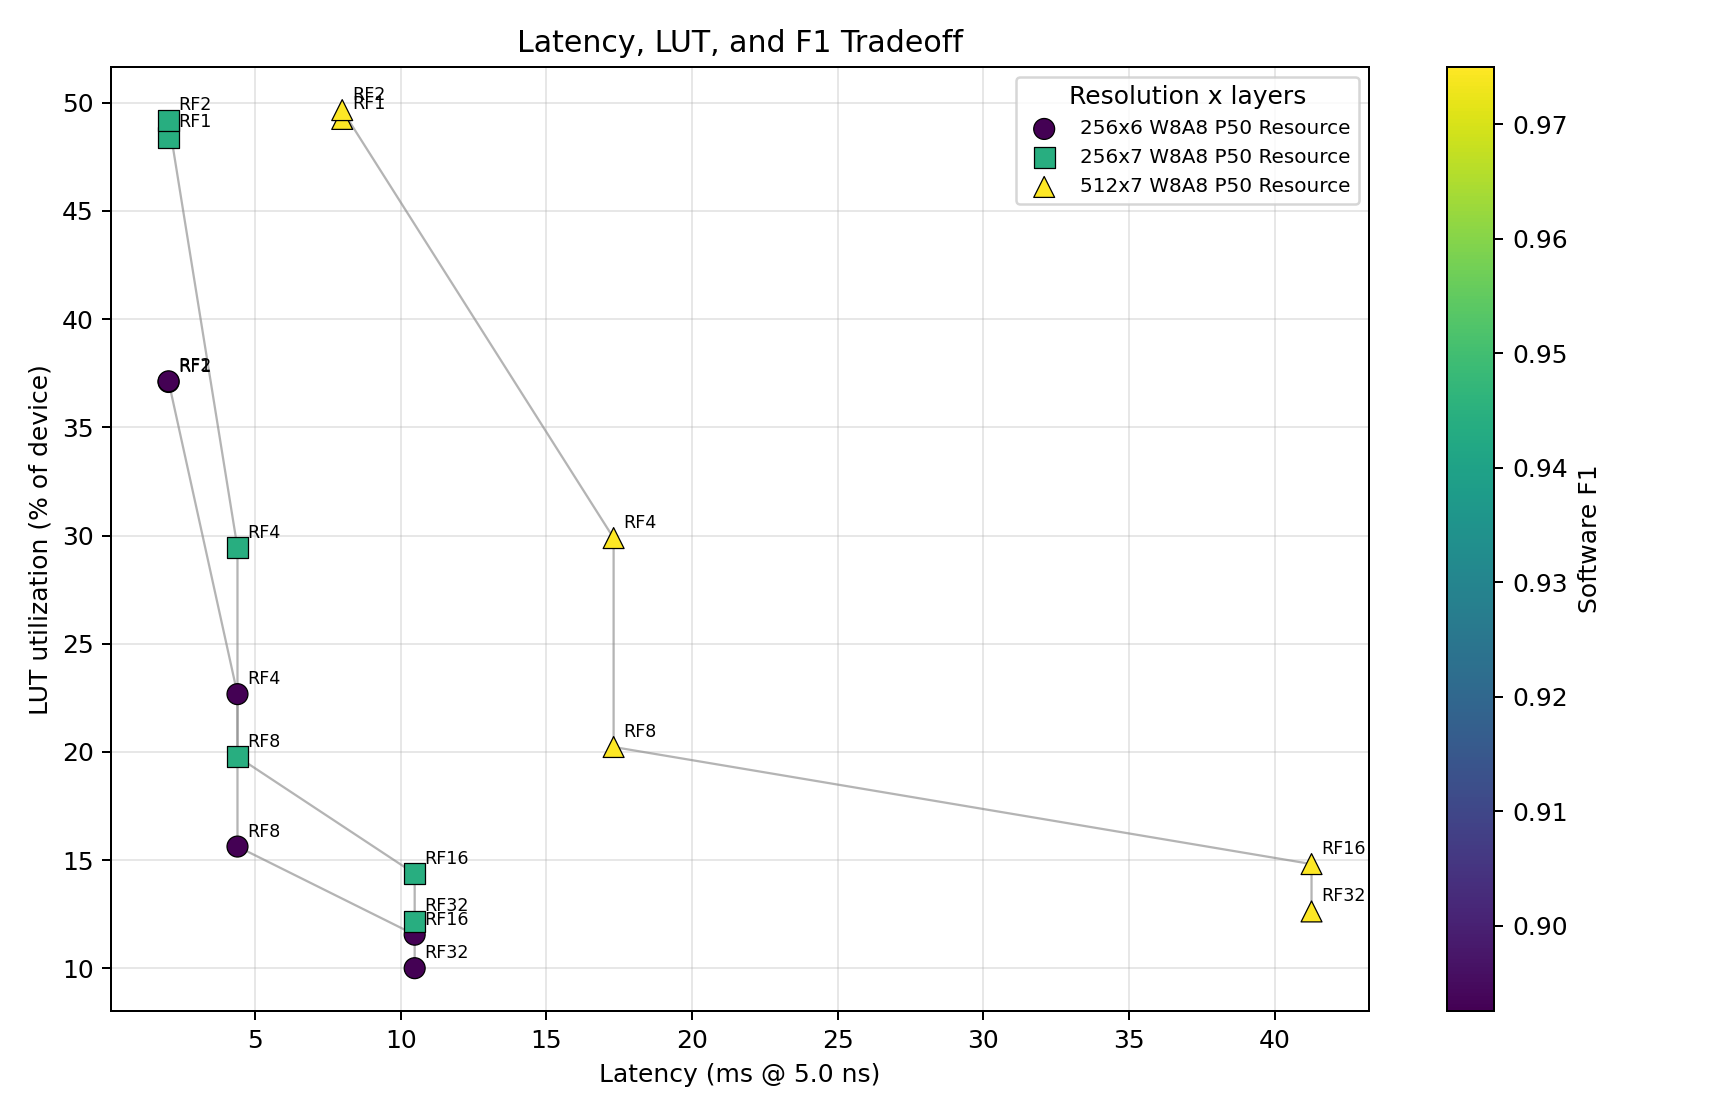
\includegraphics[width=0.92\linewidth]{figures/hls_latency_resource_f1_resource_strategy.png}
    \caption{Latency, LUT utilization, and F1 tradeoff for W8A8 P50 resource-strategy candidates. Marker shapes distinguish the 256$\times$7 and 512$\times$7 reuse-factor sweeps from the manually tuned v1 deployment candidates.}
    \label{fig:hls-tradeoff}
\end{figure}

Figure~\ref{fig:hls-latency-f1-frontier} and  Figure~\ref{fig:hls-lut-f1-frontier} show the broader design-space frontier. Unless the design is hand-optimized per CNN layer, better F1 generally requires a larger latency budget. The same pattern appears for LUT utilization. Higher-quality models are available, but they move rightward on the latency and LUT axes. The hand-optimized points are important because they shift selected candidates toward the useful frontier instead of accepting the default global resource-strategy mapping.

\begin{figure}[t]
    \centering
    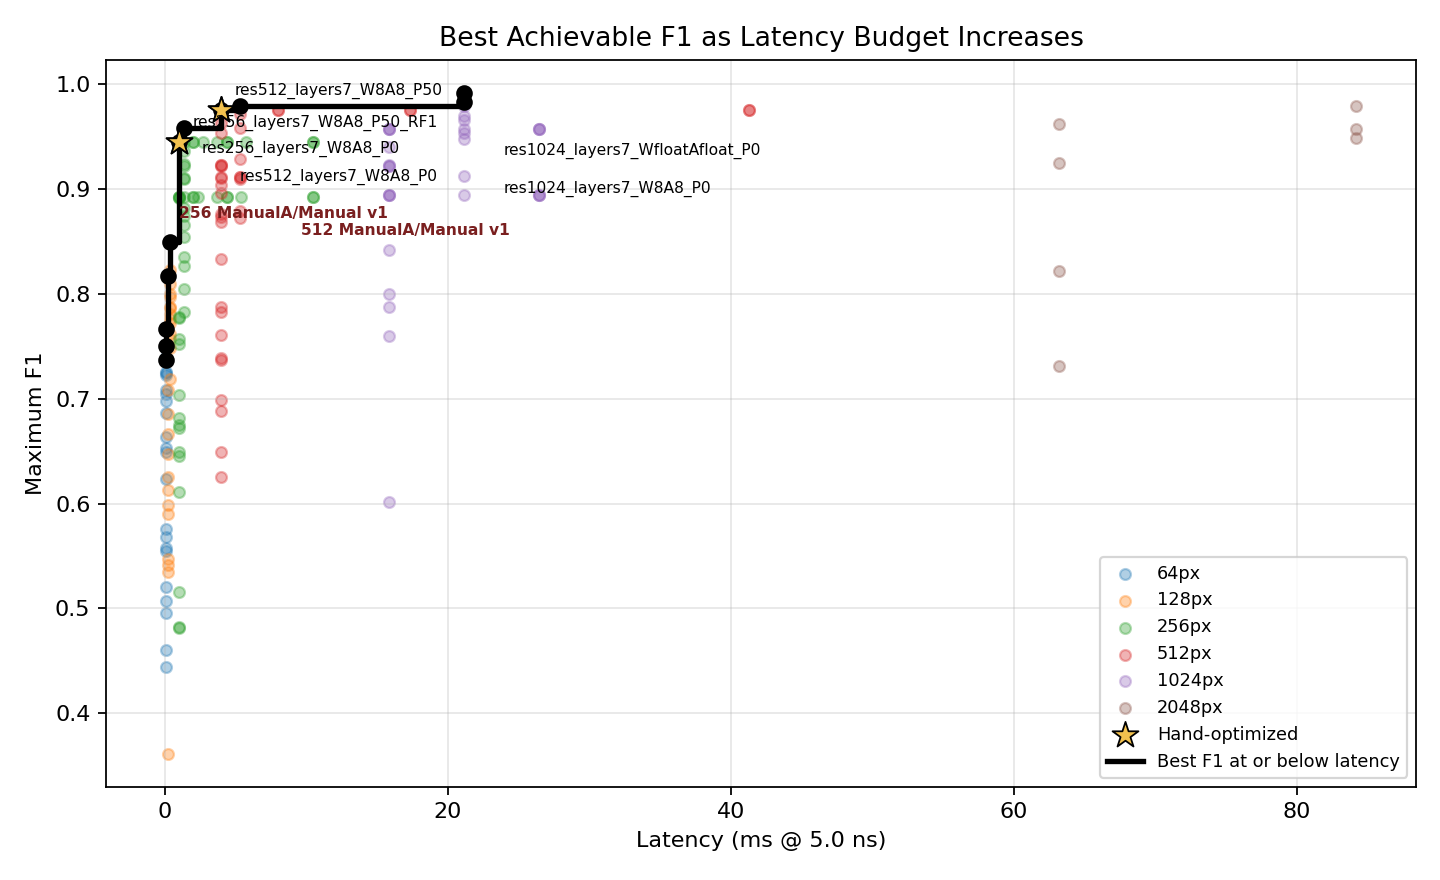
\includegraphics[
        width=\linewidth,
        trim={0 5mm 0 3mm},
        clip
    ]{figures/hls_latency_f1_frontier.png}

    \caption{
        Best achievable F1 as the latency budget increases.
        The black frontier shows the maximum F1 achieved by any synthesized
        candidate within each latency budget. Stars indicate the manually
        optimized deployment candidates.
    }
    \label{fig:hls-latency-f1-frontier}
\end{figure}

\begin{figure}[t]
    \centering
    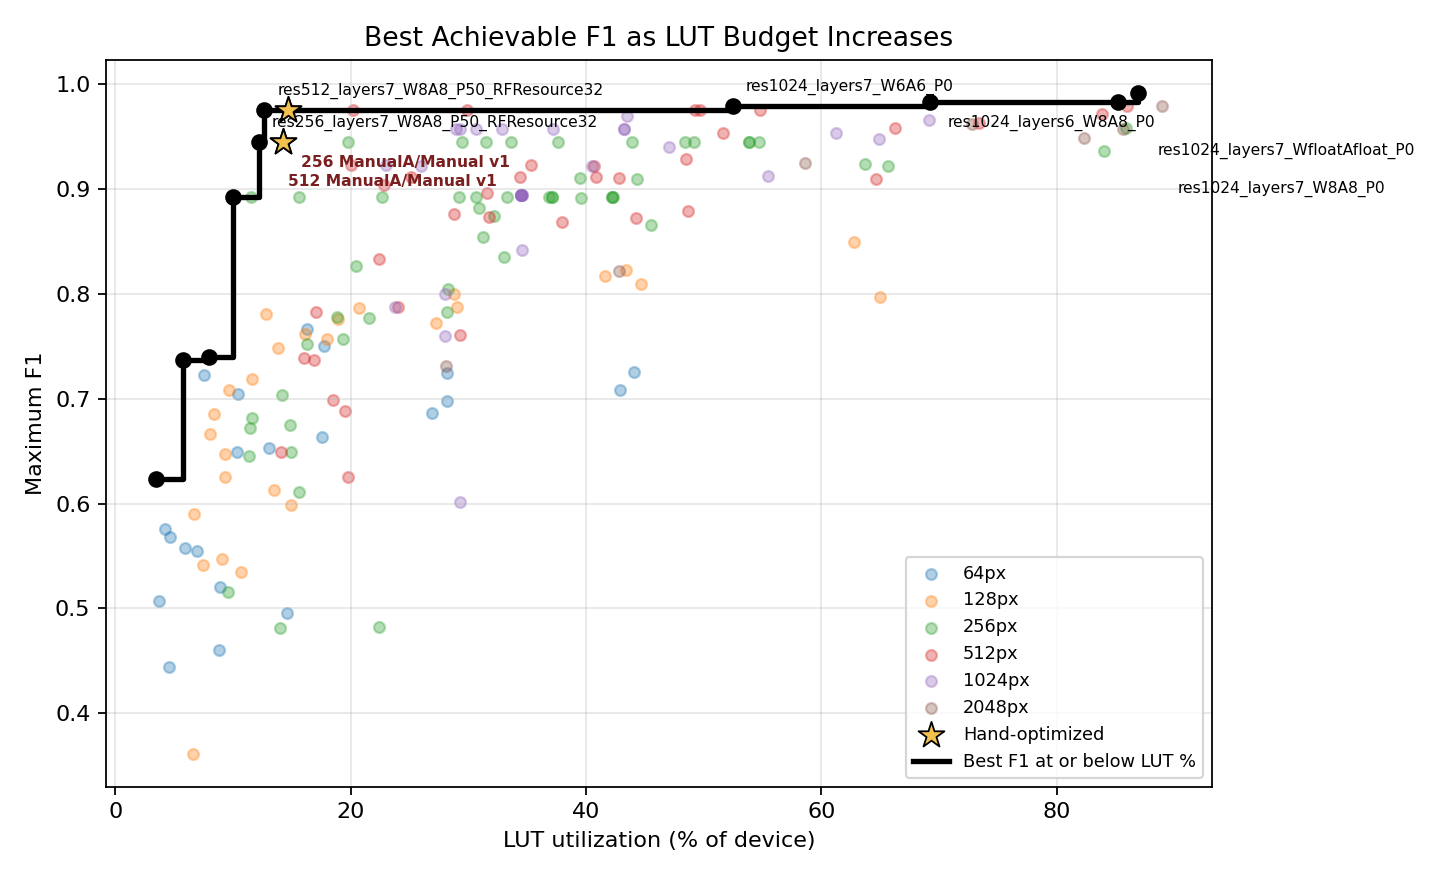
\includegraphics[
        width=\linewidth,
        trim={0 5mm 0 3mm},
        clip
    ]{figures/hls_lut_f1_frontier.png}

    \caption{
        Best achievable F1 as the LUT budget increases.
        The black frontier shows the maximum F1 achieved by any synthesized
        candidate within each LUT budget. Stars indicate the manually
        optimized deployment candidates.
    }
    \label{fig:hls-lut-f1-frontier}
\end{figure}

\section{Final Synthesized Candidates}
\label{sec:final-synthesized-candidates}

The final comparison focuses on two synthesized models. The 256$\times$7 model is the preferred deployment candidate. The 512$\times$7 model is the accuracy-oriented alternative. 

Table~\ref{tab:final-candidates} shows the final comparison. Classification metrics are evaluated on the original small-RO test set unless stated otherwise. The extended TPR is measured on the extended RO-footprint dataset.

\begin{table}[t]
    \centering
    \caption{Final synthesized candidates. Resource percentages are routed hls4ml wrapper/user-logic attribution on the target U55C.}
    \label{tab:final-candidates}
    \resizebox{\linewidth}{!}{
    \begin{tabular}{l r r r r r r r r r r}
        \toprule
        \textbf{Model} &
        \textbf{Acc.} &
        \textbf{F1} &
        \textbf{TPR} &
        \textbf{TPR Ex.} &
        \textbf{FPR} &
        \textbf{AUC} &
        \textbf{Latency} &
        \textbf{LUT} &
        \textbf{BRAM} &
        \textbf{DSP} \\
        \midrule
        % Source: ../ml_deep_bitstream_inspection/hls4ml/reproducibility/prod_res256_coyote_accel_downsampler_hls4ml_e2e_20260524/results/performance_summary.json
        256$\times$7 &
        87.7\% &
        88.5\% &
        92.0\% &
        98.7\% &
        16.9\% &
        95.1\% &
        3.35 ms &
        +4.47\% &
        +17.86\% &
        +14.72\% \\
        \midrule
        % Source: ../ml_deep_bitstream_inspection/hls4ml/reproducibility/prod_res512_coyote_accel_downsampler_hls4ml_e2e_20260524/results/performance_summary.json
        512$\times$7 &
        90.4\% &
        90.5\% &
        89.3\% &
        100.0\% &
        8.45\% &
        96.9\% &
        6.53 ms &
        +4.90\% &
        +61.78\% &
        +14.45\% \\
        \bottomrule
    \end{tabular}
    }
\end{table}

The 512$\times$7 model has higher accuracy, higher F1, lower false positive rate, higher ROC AUC, and perfect TPR on the extended RO-footprint dataset. This makes it the stronger detection candidate.

The 256$\times$7 model is the better deployment candidate. It has lower added latency and much lower BRAM overhead. Its F1 is only two percentage points lower than the 512$\times$7 model, and its original-set TPR is higher. The BRAM difference is the main reason for preferring 256$\times$7. The routed hierarchy attributes 61.78\% of device BRAM to the 512$\times$7 checker wrapper, while the 256$\times$7 wrapper accounts for 17.86\%.

\section{Latency Context}
\label{sec:latency-context}

The added inspection latency should be interpreted relative to the latency of partial reconfiguration and serverless invocation. Table~\ref{tab:latency-context} compares the 256$\times$7 and 512$\times$7 inspection latencies with F3 and generic serverless reference points~\cite{mainas2025f3,ustiugov2021stellar}.

\begin{table}[t]
    \centering
    \caption{Added inspection latency relative to deployment and serverless latency references.}
    \label{tab:latency-context}
    \begin{tabular}{p{0.46\linewidth} r r r}
        \toprule
        \textbf{Context} & \textbf{Baseline} & \textbf{256$\times$7} & \textbf{512$\times$7} \\
        \midrule
        F3 warm path with reconfiguration &
        141 ms &
        +2.38\% &
        +4.63\% \\
        \midrule
        Coyote PR on VU9P with 6\% PR region &
        6.04 ms &
        +55.46\% &
        +108.11\% \\
        \midrule
        Coyote PR on VU9P with 33\% PR region &
        36.94 ms &
        +9.07\% &
        +17.68\% \\
        \midrule
        Coyote PR on VU9P with 66\% PR region &
        73.27 ms &
        +4.57\% &
        +8.91\% \\
        \midrule
        Generic FaaS cold invocation median &
        448 ms &
        +0.75\% &
        +1.46\% \\
        \bottomrule
    \end{tabular}
\end{table}

The added latency is small relative to full serverless invocation latencies and larger PR operations. It is more significant for very small PR regions. This suggests that FPGA-resident inspection is most attractive when the checker is used in realistic deployment paths where PR and runtime overheads already dominate a few milliseconds of inference time.

The 256$\times$7 model adds 3.35 ms. The 512$\times$7 model adds 6.53 ms. Both are plausible for deployment-path inspection, but the smaller model gives a safer latency budget.

\section{Resource Context}
\label{sec:resource-context}

The baseline Coyote design uses 10.26\% of LUTs and 9.77\% of BRAM on the target device. It uses no URAM or DSPs in the reported baseline. The checker adds resources on top of this baseline.

Table~\ref{tab:resource-context} summarizes the baseline and the added checker overhead.

\begin{table}[t]
    \centering
    \caption{Baseline Coyote resource usage and routed checker wrapper/user-logic attribution.}
    \label{tab:resource-context}
    \begin{tabular}{l r r r r}
        \toprule
        \textbf{Design} & \textbf{LUT} & \textbf{BRAM} & \textbf{URAM} & \textbf{DSP} \\
        \midrule
        Baseline Coyote &
        10.26\% &
        9.77\% &
        0\% &
        0\% \\
        \midrule
        % Source: ../ml_deep_bitstream_inspection/hls4ml/reproducibility/prod_res256_coyote_accel_downsampler_hls4ml_e2e_20260524/results/performance_summary.json
        Added 256$\times$7 checker &
        +4.47\% &
        +17.86\% &
        +1.15\% &
        +14.72\% \\
        \midrule
        % Source: ../ml_deep_bitstream_inspection/hls4ml/reproducibility/prod_res512_coyote_accel_downsampler_hls4ml_e2e_20260524/results/performance_summary.json
        Added 512$\times$7 checker &
        +4.90\% &
        +61.78\% &
        +1.77\% &
        +14.45\% \\
        \bottomrule
    \end{tabular}
\end{table}

The LUT overhead is similar for both synthesized candidates. DSP overhead is also similar. BRAM is the limiting resource. This makes the 256$\times$7 candidate more attractive for integration because it leaves more memory resources available for the shell, services, and user logic.

\section{Quantization and Pruning}
\label{sec:quantization-pruning-results}

Quantization and pruning are evaluated as hardware-aware compression techniques~\cite{coelho2020qkeras,han2016deepcompression}. Quantization reduces arithmetic precision. Pruning removes weights and increases sparsity. Both can reduce the cost of a neural network, but the benefit depends on the synthesis flow and on whether the generated hardware can exploit the reduced precision or sparsity. For the selected W8A8 models, quantization is not applied only after training. We use QKeras quantization-aware training so the model learns under the target 8-bit weight and activation quantizers.

For quantized models, we check both software quality and hls4ml parity. This is important because a low-bit model can have good software accuracy but still produce mismatches after conversion. For pruned models, we track actual sparsity and classification quality. Sparse models are useful only if sparsity translates into lower synthesis cost or better feasibility.

In the final design selection, quantization and pruning are treated as supporting tools. The main deployment decision is driven by the synthesized 256$\times$7 and 512$\times$7 candidates, where measured latency and resource overhead are available.

\section{Takeaway}
\label{sec:hls4ml-takeaway}

The hardware results show that FPGA-resident CNN inspection is feasible, but the design point matters. The 512$\times$7 model gives stronger detection metrics, especially lower FPR, higher ROC AUC, and perfect TPR on the extended RO-footprint dataset. It also has much higher BRAM overhead and roughly double the latency of the 256$\times$7 model.

The 256$\times$7 model is the preferred candidate for further Coyote integration. It provides useful detection quality, lower added latency, and much lower BRAM overhead. It is the better balance between security coverage and deployment cost.
